\documentclass{article}%
\usepackage[T1]{fontenc}%
\usepackage[utf8]{inputenc}%
\usepackage{lmodern}%
\usepackage{booktabs}%
\usepackage{textcomp}%
\usepackage{lastpage}%
\usepackage{geometry}%
\usepackage{amsmath}%
\geometry{
    paper=a4paper,
    head=0cm,
    left=2cm,
    right=2cm,
    top=0cm,
    bottom=2cm,
    includehead=True,
    includefoot=True
}%
\usepackage{graphicx}%
%
\usepackage{multicol}%
\usepackage{lipsum}%
\usepackage{float}%
\usepackage{verbatim}%
\title{
    Reconstructing Arrival-Times of individual Photons
    in a continous Stream of Night-Sky-Light
}%
\author{Sebastian A. Mueller}%
\date{}%
%
\begin{document}%
\maketitle%

\newcommand{\F}{F_\text{night-sky-background}}
\newcommand{\Ftyp}{F_\text{dark-night}}
\begin{multicols}{2}%
%
The atmospheric Cherenkov-method can reconstruct the type, energy, and direction of a cosmic particle from the Cherenkov-light emitted by an air-shower.
%
Photo-sensors and read-out are cost-drivers.
%
Instruments must sense blueish Cherenkov-light, better reject reddish night-sky-light, and must reconstruct the arrival-times of the photons with $\sim{}$5\,ns resolution.
\newline
%
We expect a continues read-out into digital buffers, where each individual photon is recorded, to be beneficial for the atmospheric Cherenkov-method as it allows fast computational access to all observables.
%
We expect such a read-out to lower the energy-threshold, to improve the separation of Cherenkov- from night-sky-light, and to improve the reconstruction of the cosmic particle \cite{jung2005star,catalano2008single}.
\newline
%
One way of continues read-out are flash analog-digital-converters (ADC)s.
%
However, their cost and power-consumption scale rapidly with their sampling frequency $f$.
%
\begin{eqnarray*}
C_\text{ADC}(f) &\sim& f^2,\\
P_\text{ADC}(f) &\sim& f^2.
\end{eqnarray*}
%
In this report, we explore the usage of many slow ($f$ < 100\,MHz) ADCs.
%
We want each ADC to digitizes the signal of a photo-sensor with only little acceptance and thus a small rate of night-sky-photons.
%
We hope that when the photo-sensor's acceptance (area and solid angle) is small enough, and thus its rate of night-sky-photons is small, than a slow ADC in combination with a little computing will be able to reconstruct the arrival times of the individual photons sufficiently accurate.
%
Since the cost of silicon photo-sensors are almost only proportional to their acceptance, there is no cost overhead when replacing a big sensor with multiple small ones.
%
Since our ADCs run slow, their power-consumption and cost might still be competitive despite their large number.
%
\section*{Sensing Night-Sky-Photons}%
\label{sec:nsb}%
%
Typical photo-sensors in the atmospheric-Cherenkov method yield night-sky-photon-rates of
\begin{eqnarray*}
R_\text{PMT} &=& 144.8\times10^6\,\text{m}^{-2}\,(1^\circ)^{-2}\,\text{s}^{-1}\\
R_\text{SiPM} &=& 280.3\times10^6\,\text{m}^{-2}\,(1^\circ)^{-2}\,\text{s}^{-1}.
\end{eqnarray*}
%
The rates result out of the typical flux $\F{}$ during observations, see Figure \ref{fig:nsb}, and the corresponding photon-detection-efficiencies, see Figure \ref{fig:pde}.
%
The typical flux  corresponds to a sky surface brightness of
%
\begin{eqnarray*}
\F{} &\hat{=}& 21\,\text{mag}\,\text{arcsec}^{-2}.
\end{eqnarray*}
%
Observations take place in the range of fluxes from
\begin{eqnarray*}
0.8 &> \F{} / \Ftyp{} >& 3.
\end{eqnarray*}
%
New moon, full moon, and clouds all impact $\F{}$.
%
Figure \ref{fig:obstimeFact} shows the flux distribution during observations with a Cherenkov-telescope which tried hard to observe in the brightest conditions using silicon photo-sensors which can tolerate this stress.
%
Table \ref{TabInstrumentsNsbRates} shows the expected rates of night-sky-photons in different instruments.
%
\begin{figure}[H]%
\centering%
\includegraphics[width=1.0\linewidth]{night_sky_background.jpg}%
\caption{
The typical flux $F_\text{Night}$ of night-sky-light \cite{gaug2013night}.
Dotted line is \cite{preuss2002study}.
Gray line is a simulated and arbitrarily scaled Cherenkov-spectrum of a 5\,GeV gamma-ray in Chile at 5\,km a.s.l.
All extrapolated from 700 - 1000\,nm.
}%
\label{fig:nsb}
\end{figure}
%
\begin{figure}[H]%
\centering%
\includegraphics[width=1.0\linewidth]{photon_efficiency.jpg}%
\caption{
Dotted line is silicon-photo-multiplier (SiPM), shape according to \cite{hamamatsu2009mppc}, and scaling according to \cite{anderhub2013design}.
Extrapolated from 700 - 1000\,nm.
Dashed line is photo-multiplier-tube (PMT) \cite{toyama2013novel}
}%
\label{fig:pde}
\end{figure}
%
\begin{figure}[H]%
\centering%
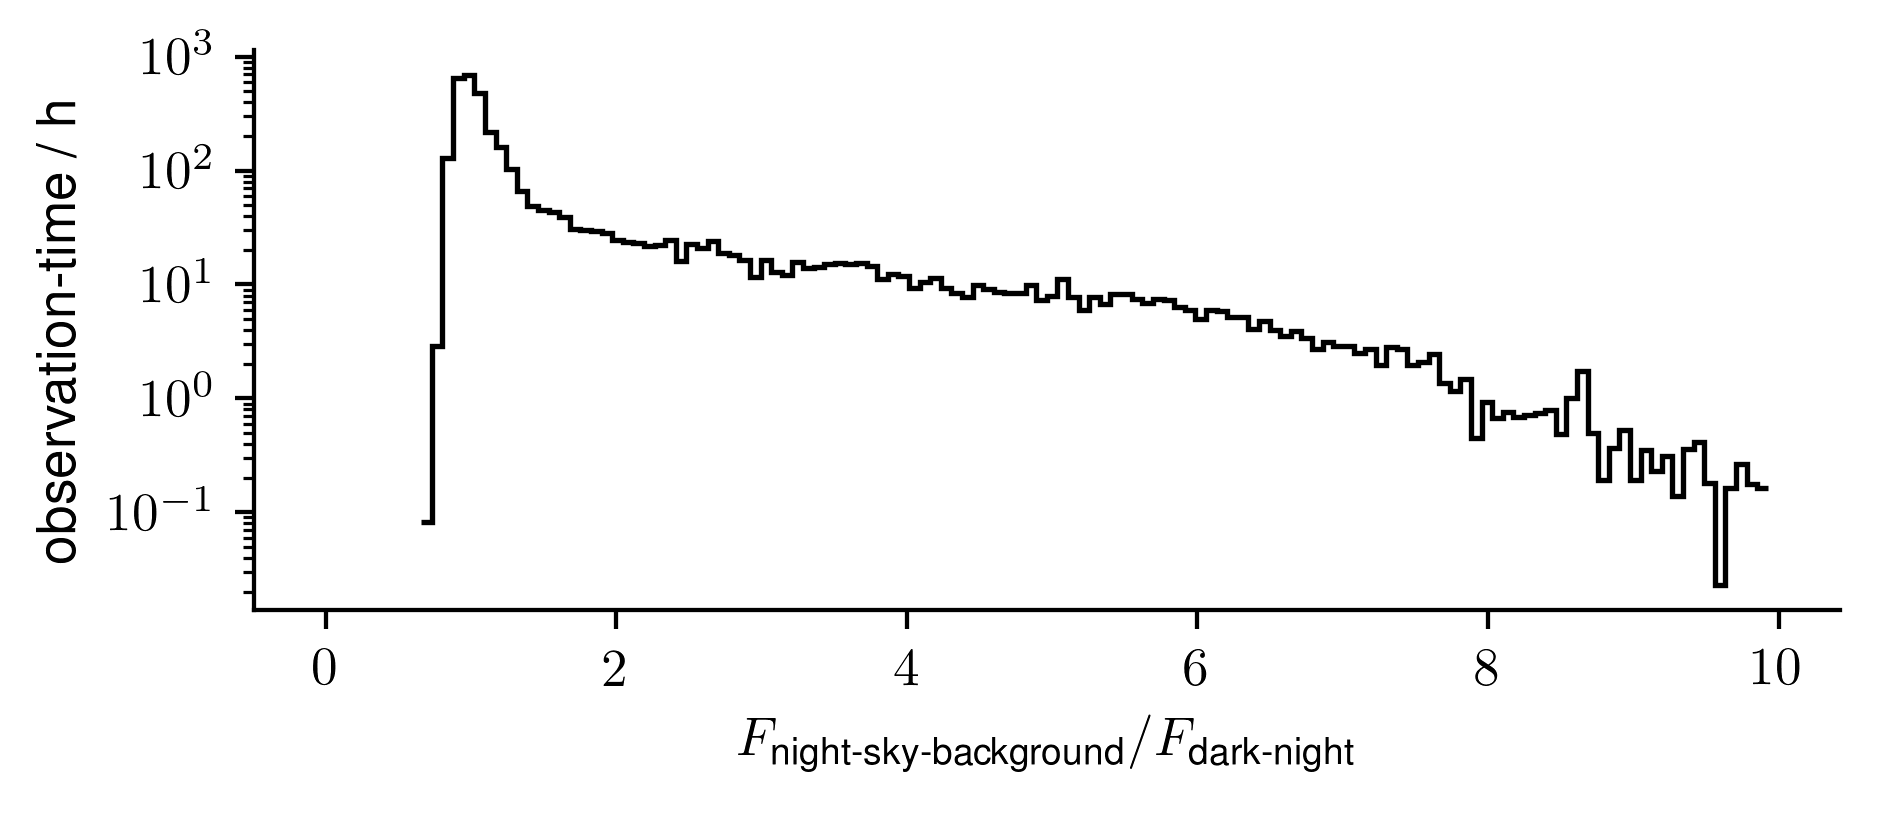
\includegraphics[width=1.0\linewidth]{observation_time_histogram.png}%
\caption{
The observations of FACT, taken from Sebastian's phd-thesis.
}%
\label{fig:obstimeFact}
\end{figure}
%
\begin{table}[H]
  \begin{center}
    \begin{tabular}{lcrrr}
        &tech.& area/ & fov/&$R$/\\
        &     & m$^2$ & $(1^\circ)^{2}$&$10^6$s$^{-1}$\\
      \hline
      FACT &SiPM& 10 & 0.01 & 29\\
      H.E.S.S. CT-1 &PMT& 108 & 0.0222 & 344\\
      H.E.S.S. CT-5 &PMT& 614 & 0.0039 & 347\\
      Portal, 71m &PMT& 65 & 0.0039 & 37\\
    \end{tabular}
    \caption{Expected rates of night-sky-photons $R$ in an individual read-out-channel (pixel or lixel).}
    \label{TabInstrumentsNsbRates}
  \end{center}
\end{table}
%
\subsection*{Filtering out night-sky-light}%
\label{SubSecFilteringOutNightSkyLight}%
%
Mirrors, lenses, and windows can provide additional filtering of reddish night-sky-light, see Figure \ref{FigNsbFilter}.
%
Table \ref{TabFilters} shows the rate $R$ for night-sky-photons when the sensors are behind mirrors and/or transmissive filters.
%
\begin{figure}[H]%
\centering%
\includegraphics[width=1.0\linewidth]{nsb_filters.jpg}%
\caption{
Dashed line is CTA's dielectric mirror for the MST, after degrading \cite{pareschi2013status,pareschi2013statusarxiv}.
%
Dotted line is VERITAS' night-sky-filter \cite{archambault2017gamma}.
%
Both Extrapolated from 700\,nm to 1000\,nm.
}%
\label{FigNsbFilter}
\end{figure}
%
\begin{table}[H]
  \begin{center}
    \begin{tabular}{cccrr}
              & \footnotesize{mirror} & \footnotesize{filter} & $R_\text{nsb}$ /   & $\eta_\text{Cer.}$ / \\
              &        &        & \footnotesize{$10^6\,\text{m}^{-2}\,(1^\circ)^{-2}\,\text{s}^{-1}$} & \footnotesize{$10^{-3}$} \\
        \hline
        PMT &             &             & 144.8 & 213\\
        .   & $\bullet{}$ &             & 135.8 & 206\\
        .   & $\bullet{}$ & $\bullet{}$ &  15.9 &  53\\
        \hline
        SiPM &             &             & 280.3 & 198\\
        .    & $\bullet{}$ &             & 188.5 & 176\\
        .    & $\bullet{}$ & $\bullet{}$ &   7.1 &  24\\
    \end{tabular}
    \caption{}
    \label{TabFilters}
  \end{center}
\end{table}
%
\section*{Simulating}%
\label{SecSimulating}%
%
\bibliographystyle{apalike}%
\bibliography{references}%
\end{multicols}{2}%
\end{document}
